\documentclass[a4paper,12pt]{article}           %   A4, pt changes regular font size
\frenchspacing                                  %   Finnish spacing
\usepackage{a4wide}                             %   Less margis
\usepackage[british]{babel}                     %   Edit this to match your language, e.g., finnish
\usepackage{xcolor}                             %   color support
    \definecolor{my_grey}{HTML}{7F7F7F}
\usepackage{icomma}                             %   Better comma in eqs. if used
\usepackage{hyperref}                           %   Clickable URLs
\usepackage{booktabs}                           %   Better tables
\usepackage{siunitx}                            %   Physics unit stuff
\usepackage{listings}                           %   Better tables
\usepackage{graphicx}                           %   Figures work
\usepackage{fontspec}                           %   Better way to handle custom fonts
\usepackage{amsmath}                            %   Basic math
\usepackage{esint}                              %   Various fancy integral symbols
\usepackage[capitalise]{cleveref}               %   \cref better than \ref
    \crefname{section}{Sec.}{Secs.}             %   Add abbreviation for Sections
\usepackage[position=top]{subfig}
    \captionsetup[subfigure]{position=top, labelfont=bf,textfont=normalfont,singlelinecheck=off,justification=raggedright}
\captionsetup[subfigure]{subrefformat=simple,labelformat=simple,listofformat=subsimple}
\renewcommand\thesubfigure{(\alph{subfigure})}
\usepackage{sectsty}                            %   Edit section titles
    %\allsectionsfont{\normalfont\sffamily}     %   ALL titles use sans-serif
    \sectionfont{\normalfont\sffamily\large\color{my_grey}} 
    \subsectionfont{\normalfont\sffamily\normalsize\color{my_grey}} 
    \subsubsectionfont{\normalfont\sffamily\small\color{my_grey}}
\setsansfont{URW Gothic L}[
    Path = fonts/,
    Extension =.ttf,
    UprightFont = * Regular,
    ItalicFont = * Italic,
    BoldFont = * Bold,
    BoldItalicFont= * Bold Italic]
\setmonofont{Source Code Pro}[
    Path = fonts/,
    Extension =.ttf,
    UprightFont = *-Regular,
    ItalicFont = *-Italic,
    BoldFont = *-Bold,
    BoldItalicFont= *-BoldItalic
]
\setmainfont{AdobeTextPro}[
    Scale = 0.958,
    Path = fonts/,
    Extension =.ttf,
    UprightFont = *-Regular,
    ItalicFont = *-It,
    BoldFont = *-Bold,
    BoldItalicFont= *-BoldIt]
\usepackage[libertine]{newtxmath}               %   Matching math font
\usepackage{fancyhdr}                           %   Nice header and footer header (and/or footer)
    \pagestyle{fancy}                               %   Makes package work
\usepackage[section]{placeins}                  %   Figures stay in declared section
\usepackage{minted}                             %   Beautiful verbatim code
    \usemintedstyle{emacs}                          %   code style
    \setminted{
        frame=lines,
        framesep=2mm,
        baselinestretch=0.9,
        fontsize=\footnotesize,
        linenos,
        breaklines
    }
\usepackage{csquotes}                           %   Correct quotes for babel
\usepackage[backend=biber,
            style=ieee,
            urldate=long,
            maxnames=5,
            dateabbrev=false]{biblatex}         %   Citation style with biblatex
\DeclareSourcemap{                              %   No ISSN for journals
    \maps[datatype=bibtex]{
        \map{
        \step[fieldset=issn, null]
        }
    }
}
\renewbibmacro*{doi+eprint+url}{                %   Print URL iff no doi
    \printfield{doi}
    \newunit\newblock{}
    \iftoggle{bbx:eprint}{
        \usebibmacro{eprint}
    }{}
    \newunit\newblock{}
    \iffieldundef{doi}{
        \usebibmacro{url+urldate}}
        {}
}

\hypersetup{
    pdfauthor={Niko Savola},                    %   Author here
}

\linespread{1.1}
\setlength{\headheight}{15pt}                   %   Suppress height warnings
\addtolength{\topmargin}{-2.4pt}


% Set commonly used math commands here
\newcommand*{\pd}[3][]{\ensuremath{\frac{\partial^{#1} #2}{\partial #3}}}
\newcommand*{\dt}[3][]{\ensuremath{\frac{\textrm{d}^{#1} #2}{\textrm{d} #3}}}
\newcommand{\dbar}{\textrm{d}\hspace*{-0.08em}\bar{}\hspace*{0.1em}}
\newcommand{\de}{\textrm{d}}
\newcommand{\sref}[1]{\textbf{\small\subref{#1}}}
\newcommand{\ve}[1]{\textbf{#1}}
\newcommand{\e}{\mathrm{e}}

\addbibresource{references.bib}
\hypersetup{
    pdftitle={Machine learning with many-body tensor networks | Niko Savola},
}
%   header
\lhead{\textsf{Special exercise}}
\chead{\textsf{PHYS-E0421 - Solid-State Physics}}
\rhead{\textsf{Niko Savola \textbf{653732}}}
%   footer
\lfoot{}
\cfoot{}
\rfoot{\thepage}


\usepackage[braket, qm]{qcircuit}  % Qiskit output
% \usepackage{titlesec}
% \titlespacing*{\section}
% {0pt}{0.7\baselineskip}{0.3\baselineskip}
% \titlespacing*{\subsection}
% {0pt}{0.65\baselineskip}{0.3\baselineskip}
% \titlespacing*{\subsubsection}
% {0pt}{0.65\baselineskip}{0.3\baselineskip}


\begin{document}

\begin{titlepage}
    {\sffamily
    \noindent
    \fontsize{12}{14}\selectfont
    Aalto University \newline
    School of Science \newline
    Department of Applied Physics

    \vspace{40mm}

    \noindent
    \fontsize{14}{16}\selectfont
    \emph{Niko Savola}

    \vspace{10mm}

    \noindent
    \fontsize{18}{22}\selectfont
    \textbf{Machine learning with many-body tensor networks}\\

    \fontsize{12}{14}\selectfont
    \noindent
    Submitted for approval: \today

    \vspace{70mm}

    \noindent
    Special exercise \\[4mm]
    PHYS-E0421 \textendash{} Solid-State Physics \\[4mm]
    } % end of \sffamily

\end{titlepage}
\newpage


\section{Introduction}

Tensor networks have been originally developed for efficiently storing and manipulating high-dimen\-sional quantum many-body states~\cite{PhysRevLett.69.2863}. These variational families of wavefunctions emerge from low-entanglement representations of quantum states. Contemporary applications however include a wide range of fields, such as, machine learning~\cite{Roberts2019}, statistical mechanics~\cite{Levin_2007}, quantum chemistry~\cite{White1999}, and cosmology~\cite{Bao_2017}.
This exercise aims to present the theory behind tensor networks and their use in machine learning. Then we present a numerical example for training a tensor network representing a quantum circuit, effectively pre-training a quantum computer for solving a problem.

% can be used in 
% https://youtu.be/q8UTwdjS95k


\section{Theory}

\subsection{Tensor networks}

Tensor networks (TN) are a powerful tool for splitting a high-dimensional function into constituent parts of smaller tensors. 
Here a tensor refers to a multidimensional array, rank zero corresponding to a scalar, rank one to a vector, rank two to a matrix, and further ranks being referred to as rank $n$ tensors.
It is natural to use Tensor network notation (TNN), which can be considered a graphical generalisation of Einstein summation~\cite{Bridgeman_2017}. This notation maps tensors to  nodes with $n$ lines corresponding to the rank $n$ of the tensor. The lines represent indices for the multidimensional array as demonstrated in \cref{sfig:tensor_basics}.

The elegance of TNN arises from contracting tensors. Multiplication is done by linking the lines of the tensors. For example, matrix-vector multiplication consists of linking a node with one line to a node with two lines. The ensuing tensor will have one free line, resulting in a vector as expected.
This logic is further demonstrated for a few examples in \cref{sfig:tensor_samples}.
Notice how multiplication of high-rank tensors is rendered graphically trivial. This is indeed useful for representing complex TN architectures.



\begin{figure}[htb]
    \centering
    \subfloat[]{{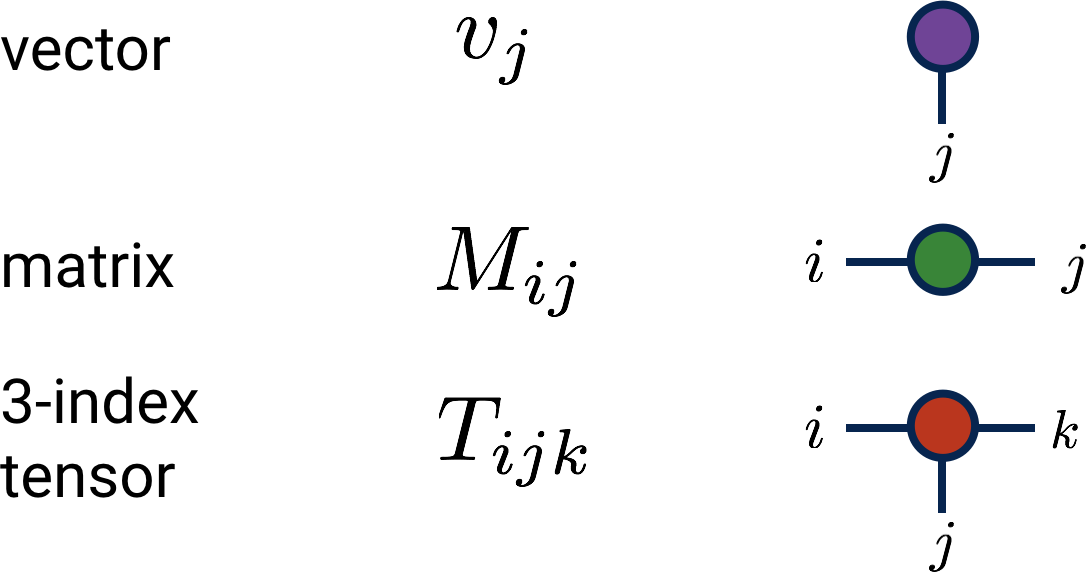
\includegraphics[width=0.43\textwidth]{figures/tensor_diagrams.png}\label{sfig:tensor_basics}}} \qquad
    \subfloat[]{{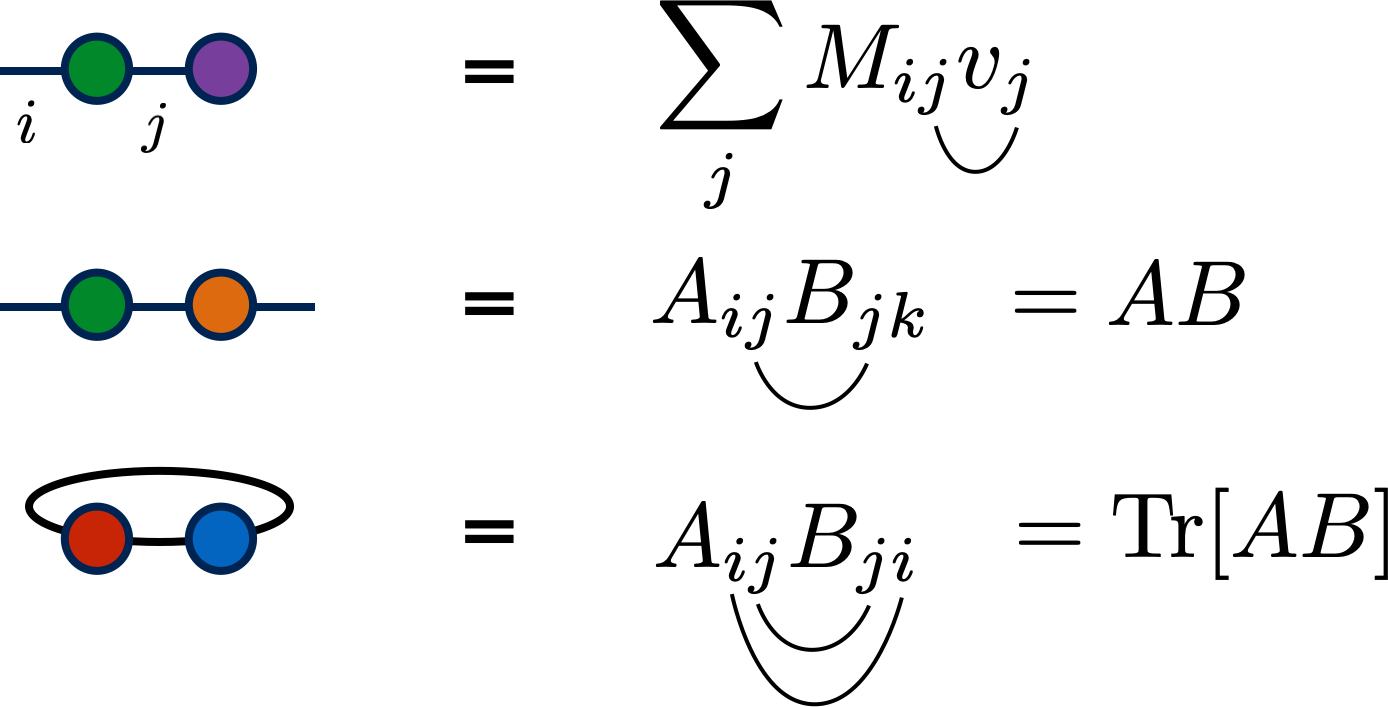
\includegraphics[width=0.45\textwidth]{figures/sample_contractions.png}\label{sfig:tensor_samples}}}
    
    \caption{\protect\subref{sfig:tensor_basics} Examples of low-rank tensors and their TNN representations. \protect\subref{sfig:tensor_samples} Examples of tensor contraction for matrices. From top to bottom: matrix-vector product, matrix multiplication, and their trace. Note how the last example results in a scalar. Schematics from Ref.~\cite{Stoudenmire2021}}
    \label{fig:tensor_diagrams}
\end{figure}


\subsubsection{Machine learning}

As popularity of deep learning has risen rapidly~\cite{DL_review}, interest in using TN as replacements or in conjunction with neural networks (NN) has also been explored.
Although TN are still an active research topic, some prominent TN factorisation architectures for machine learning have emerged, including Matrix Product States (MPS). % and Tensor Renormalization Group (TRG).
In fact, it has been shown that there exists a mapping from neural networks referred to as Restricted Boltzmann machines to TNs, highlighting the link to deep learning~\cite{PhysRevB.97.085104}.

Arguably, the best-understood tensor network decomposition is MPS. It factorises a tensor of any rank to a chain of rank three tensors, allowing one to efficiently optimize weights of any tensors for machine learning~\cite{Bridgeman_2017}. In this exercise however, we will refrain from using MPS as our system size will be small enough to optimise with methods not made specifically for TNs.



\subsection{Modelling many-body physics}

As system Hamiltonians can often be represented with Kronecker products of matrices in some basis, it is natural that they can be used with TN. Solving these Hamiltonians is done elegantly by contracting TN Ansätze to the Hamiltonian, effectively merely combining the free lines in the tensors~\cite{Bridgeman_2017}. Of course, the actual contraction computations may be difficult, yet the TNN solution remains trivial.


% https://quimb.readthedocs.io/en/latest/examples/ex_tn_train_circuit.html
\section{Example: Training a quantum circuit}

In this numerical example, we train a quantum circuit to simulate short time evolution of the quantum transverse field Ising model~\cite{Cervera-Lierta2018}. This is done with unitary TN, which can easily be converted to quantum gate operations. The unitarity is ensured with local unitary tensors $v$ obeying $v^\dagger v = vv^\dagger = I$ for an identity tensor of the corresponding rank~\cite{Haghshenas2021}.
% In fact, both also a paradigm called differentiable programming.

% \subsection{Implementation}

We use an ansatz circuit consisting of quantum U gates and Controlled-Z gates (CZ). The U-gates represent all possible single-qubit operations and are of the form
\begin{align}
    U(\theta, \phi, \lambda) =
            \begin{pmatrix}
                \cos\left(\frac{\theta}{2}\right)          & -e^{i\lambda}\sin\left(\frac{\theta}{2}\right) \\
                e^{i\phi}\sin\left(\frac{\theta}{2}\right) & e^{i(\phi+\lambda)}\cos\left(\frac{\theta}{2}\right)
            \end{pmatrix}
            ,
\end{align}
whereas the CZ gates are two-qubit gates flipping the phase if one of the qubits is in the $|1\rangle$ state. It is a symmetric operation and is represented as
\begin{align}
    CZ=
        |0\rangle\langle 0| \otimes I + |1\rangle\langle 1| \otimes \sigma_\text{z} =
        \begin{pmatrix}
            1 & 0 & 0 & 0 \\
            0 & 1 & 0 & 0 \\
            0 & 0 & 1 & 0 \\
            0 & 0 & 0 & -1
        \end{pmatrix}
        ,
\end{align}
where $\sigma_\text{z}$ is a Pauli-Z gate.
Our ansatz is implemented numerically in Python using the \emph{quimb} library~\cite{Gray2018} as
\setminted[python]{fontsize=\scriptsize}
\begin{minted}{python}
import quimb as qu
import quimb.tensor as qtn

n = 5
depth = 4
circ = qtn.Circuit(n)

for d in range(depth):
    for i in range(circ.N):
        params = qu.randn(3, dist='uniform')  # initialize with random parameters
        circ.apply_gate('U3', *params, i, gate_round=d, parametrize=True)

    for i in (reversed(regs) if (d % 2 == 0) else regs):
        circ.apply_gate('CZ', i, i + 1, gate_round=d)

for i in range(circ.N):  # final single qubit layer
    params = qu.randn(3, dist='uniform')  # initialize with random parameters
    circ.apply_gate('U3', *params, i, gate_round=r, parametrize=True)
\end{minted}
The resulting ansatz consists of exclusively tensors. Thus, a graph complying with TNN presented in \cref{fig:tensor_diagrams} can be generated and is shown in \cref{fig:TNN_circuit} with colouring displaying the quantum gates and qubit indices in \protect\subref{sfig:TNN} and \protect\subref{sfig:TNN_qubits}, respectively.
\begin{figure}[tb]
    \centering
    \subfloat[]{{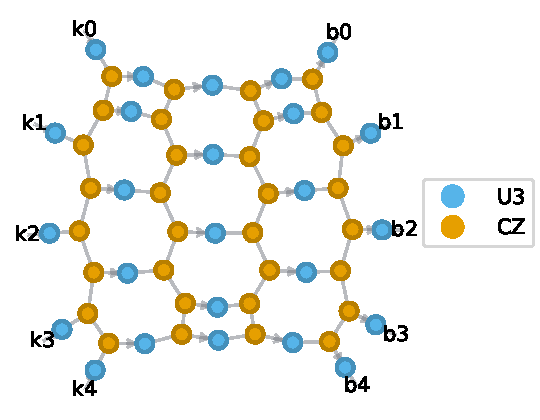
\includegraphics[width=0.42\textwidth]{figures/tensor_network_graph.pdf}\label{sfig:TNN}}} \quad
    \subfloat[]{{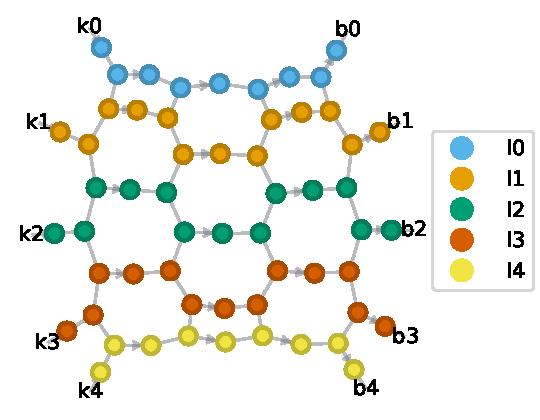
\includegraphics[width=0.42\textwidth]{figures/tensor_network_qubits.pdf}\label{sfig:TNN_qubits}}}
    
    \caption{TNN graph of our ansatz quantum circuit with colouring for \protect\subref{sfig:TNN} quantum gates \protect\subref{sfig:TNN_qubits} qubit indices. The open ends of the TN, labelled with \texttt{k} and \texttt{b}, are consequently linked to a target problem.}
    \label{fig:TNN_circuit}
\end{figure}
The free lines of the TN are consequently connected to a unitary matrix representing the short time evolution of the transverse field Ising model $U(t) = \e^{-itH}$.
This is the target unitary matrix we are trying to replicate with the ansatz.
We implement this in quimb for $t=2$ as follows:
\begin{minted}{python}
H = qu.ham_ising(n, cyclic=False)
U = qtn.Tensor(data=(U_dense := qu.expm(-1j * (t := 2) * H)).reshape([2] * (2 * n)), inds=[f'k{i}' for i in range(n)] + [f'b{i}' for i in range(n)], tags={'U_TARGET'})
\end{minted}

Our \emph{loss function} to minimise, i.e., the objective of the model is 
\begin{align}
    L(H_\text{ansatz}) = 1 - \left|\left(H_\text{ansatz}\right)_\gamma U^\gamma \right|
    ,
\end{align}
where $\gamma$ denotes indices for tensor contraction with \emph{tensor index notation}~\cite{Haghshenas2021}.
We accelerate the training with JAX~\cite{jax2018github}, a framework for automatic differentiation and a just-in-time compiler for graphics processing units (GPU). Limited-memory BFGS (L-BFGS) is chosen as the optimization algorithm~\cite{zhu1997algorithm}. Additionally, basin-hopping is used to avoid local minima by adding random perturbations found minima.



\subsection{Results}

The training was performed using an NVIDIA RTX 3070 GPU for the ansatz circuit with five qubits and four layers of $U$-gate rotations per qubit as shown in \cref{sfig:TNN}.
As the system size was not large, it was possible to solve the exact time evolution of the state $U(t)$ and compare it to the evolution provided by the trained ansatz. This was done for randomly-initialised states $|\psi\rangle$ by estimating the \emph{fidelity} of the ansatz. As our states are pure, we can define the fidelity to be $\langle U^* \psi | H_\text{ansatz} \psi \rangle$. For this value, we attained 98.94\% from 1000 random trials. Thus, the ansatz time evolution appears competent.

\begin{figure}[htb]
    \centering
    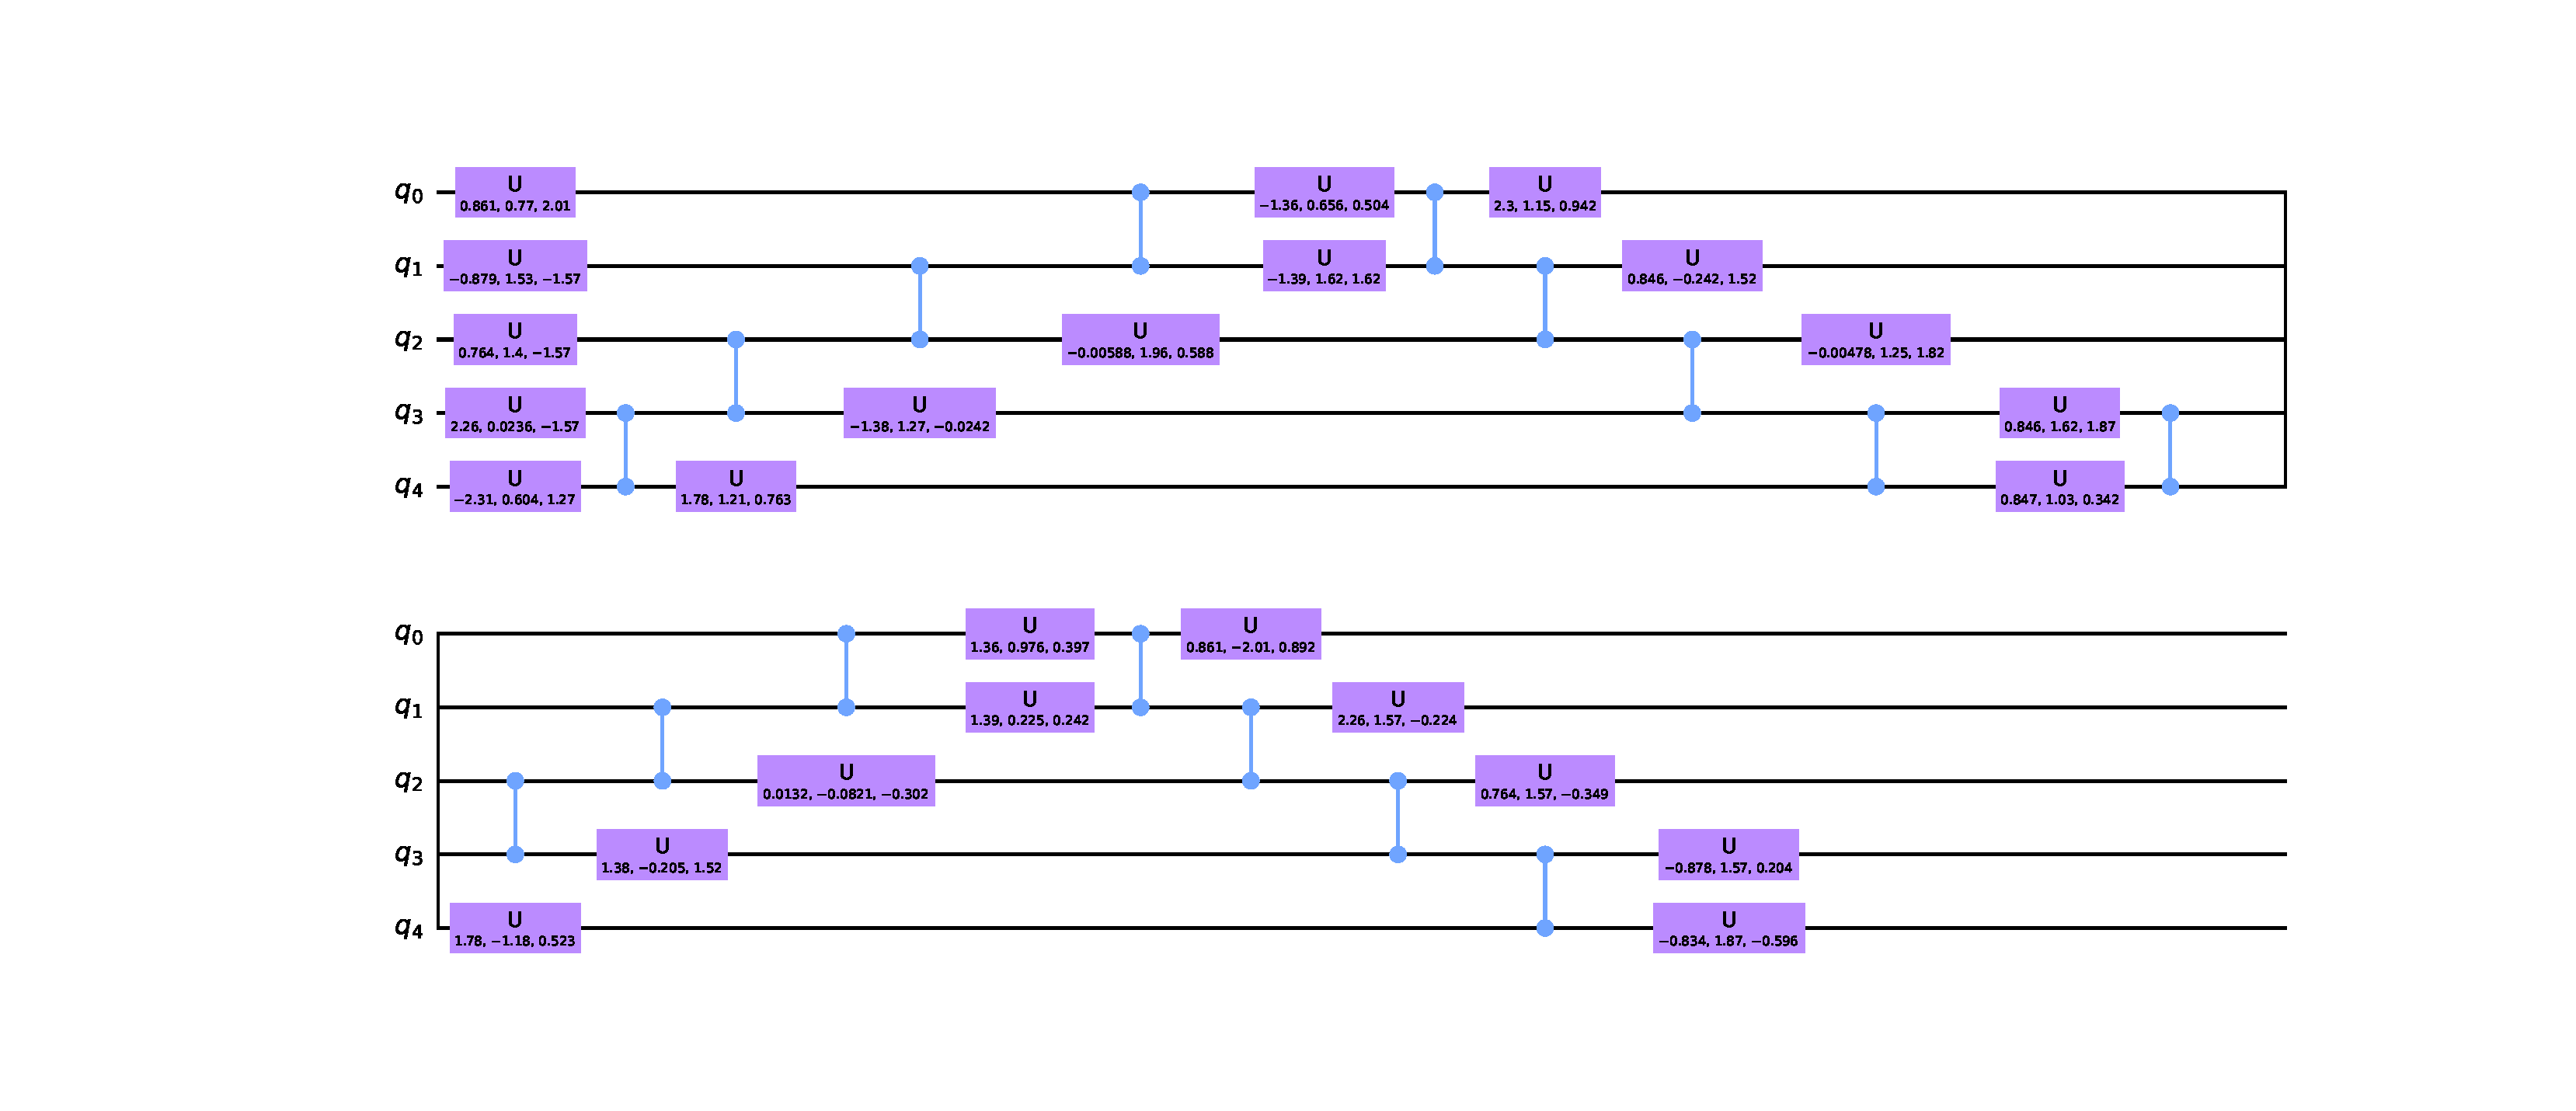
\includegraphics[width=0.97\textwidth]{figures/ansatz_circuit.pdf}
    \caption{Result of the trained quantum ansatz circuit generated with Qiskit~\cite{Qiskit}. The purple blocks represent U-gates with the given $\theta, \phi,$ and $\lambda$ parameters while the blue lines with dots are CZ-gates.}
    \label{fig:qasm_circuit}
\end{figure}

Ultimately, the trained TN was converted back to unitary matrices for quantum circuits. This final circuit is depicted graphically in \cref{fig:qasm_circuit}. As quantum computers with five or more qubits have already been realised~\cite{VTT-IQM}, this circuit could be run on actual quantum hardware. Although it would typically first require transpilation to a native gateset from the general $U$-gates in the noisy inter\-mediate-scale quantum era (NISQ)~\cite{Wilson2020,Li2020}.


\newpage
\section{Conclusions}

Considering the high fidelity for the states, it is safe to assume that five qubits can already simulate the short time evolution of the Ising model. The accuracy could however be improved with circuit depth and by increasing the training and circuit execution times. 

For NISQ devices, it would be interesting to check whether a limited gate set would perform satisfactorily, allowing co-designed quantum computers~\cite{Algaba2022} with hardcoded gates for a given problem. Additionally, examining whether the model generalises for time evolution of similar systems, like the Heisenberg J1-J2 model, should be considered along with long time evolution in the future.





%-------------------
%   Bibliography
%-------------------

% \newpage
% \thispagestyle{empty}
\setlength\bibitemsep{0.0\baselineskip}
\addcontentsline{toc}{section}{References}
\renewcommand*{\bibfont}{\fontsize{8.5pt}{10.7pt}\selectfont}  %TODO
\printbibliography{}


\end{document}
